%%%%%%%%%%%%%%%%%%%%%%%%%%%%%%%%%%%%%%%%%%%%%
%%%%%                                   %%%%%
%%%%%       2014.8.29,   afternoon      %%%%%
%%%%%          1.1st version            %%%%%
%%%%%                                   %%%%%
%%%%%%%%%%%%%%%%%%%%%%%%%%%%%%%%%%%%%%%%%%%%%
\RequirePackage{lineno}
%\documentclass[prd,amsmath,amssymb,showpacs,superscriptaddress,nofootinbib,twocolumn]{revtex4}
\documentclass[prd,amsmath,amssymb,showpacs,superscriptaddress,nofootinbib]{revtex4}
\usepackage{graphicx}
\usepackage{epsfig}
\usepackage{dcolumn}
\usepackage{bm}
\usepackage{overpic}
\setlength{\parskip}{0\baselineskip}
\newcommand{\ra}{\rightarrow}
\newcommand{\BR}{{\cal B}}
\newcommand{\eff}{\varepsilon}
\newcommand{\LL}{\ell^+\ell^-}
\newcommand{\jpsi}{J/\psi}
\newcommand{\pio}{\pi^{0}}
\newcommand{\pip}{\pi^{+}}
\newcommand{\pim}{\pi^{-}}
\newcommand{\etap}{\eta^{\prime}}
\newcommand{\chisq}{\chi^{2}}
\renewcommand{\thefootnote}{\fnsymbol{footnote}}
\pagewiselinenumbers
\begin{document}

\normalsize
\parskip=0pt plus 1pt minus 1pt

\title{\boldmath Dalitz plot analyses of $\eta/\etap \ra 3\pi$  }

\author{
M.~Ablikim$^{1}$, M.~N.~Achasov$^{8,a}$, X.~C.~Ai$^{1}$, O.~Albayrak$^{4}$, M.~Albrecht$^{3}$, D.~J.~Ambrose$^{42}$, A.~Amoroso$^{46A,46C}$, F.~F.~An$^{1}$, Q.~An$^{43}$, J.~Z.~Bai$^{1}$, R.~Baldini Ferroli$^{19A}$, Y.~Ban$^{29}$, D.~W.~Bennett$^{18}$, J.~V.~Bennett$^{4}$, M.~Bertani$^{19A}$, D.~Bettoni$^{20A}$, J.~M.~Bian$^{41}$, F.~Bianchi$^{46A,46C}$, E.~Boger$^{22,g}$, O.~Bondarenko$^{23}$, I.~Boyko$^{22}$, S.~Braun$^{38}$, R.~A.~Briere$^{4}$, H.~Cai$^{48}$, X.~Cai$^{1}$, O. ~Cakir$^{37A}$, A.~Calcaterra$^{19A}$, G.~F.~Cao$^{1}$, S.~A.~Cetin$^{37B}$, J.~F.~Chang$^{1}$, G.~Chelkov$^{22,b}$, G.~Chen$^{1}$, H.~S.~Chen$^{1}$, J.~C.~Chen$^{1}$, M.~L.~Chen$^{1}$, S.~J.~Chen$^{27}$, X.~Chen$^{1}$, X.~R.~Chen$^{24}$, Y.~B.~Chen$^{1}$, H.~P.~Cheng$^{16}$, X.~K.~Chu$^{29}$, Y.~P.~Chu$^{1}$, G.~Cibinetto$^{20A}$, D.~Cronin-Hennessy$^{41}$, H.~L.~Dai$^{1}$, J.~P.~Dai$^{1}$, D.~Dedovich$^{22}$, Z.~Y.~Deng$^{1}$, A.~Denig$^{21}$, I.~Denysenko$^{22}$, M.~Destefanis$^{46A,46C}$, F.~De~Mori$^{46A,46C}$, Y.~Ding$^{25}$, C.~Dong$^{28}$, J.~Dong$^{1}$, L.~Y.~Dong$^{1}$, M.~Y.~Dong$^{1}$, S.~X.~Du$^{50}$, J.~Z.~Fan$^{36}$, J.~Fang$^{1}$, S.~S.~Fang$^{1}$, Y.~Fang$^{1}$, L.~Fava$^{46B,46C}$, F.~Feldbauer$^{21}$, G.~Felici$^{19A}$, C.~Q.~Feng$^{43}$, E.~Fioravanti$^{20A}$, C.~D.~Fu$^{1}$, Q.~Gao$^{1}$, Y.~Gao$^{36}$, I.~Garzia$^{20A}$, C.~Geng$^{43}$, K.~Goetzen$^{9}$, W.~X.~Gong$^{1}$, W.~Gradl$^{21}$, M.~Greco$^{46A,46C}$, M.~H.~Gu$^{1}$, Y.~T.~Gu$^{11}$, Y.~H.~Guan$^{1}$, L.~B.~Guo$^{26}$, T.~Guo$^{26}$, Y.~P.~Guo$^{21}$, Z.~Haddadi$^{23}$, S.~Han$^{48}$, Y.~L.~Han$^{1}$, F.~A.~Harris$^{40}$, K.~L.~He$^{1}$, M.~He$^{1}$, Z.~Y.~He$^{28}$, T.~Held$^{3}$, Y.~K.~Heng$^{1}$, Z.~L.~Hou$^{1}$, C.~Hu$^{26}$, H.~M.~Hu$^{1}$, J.~F.~Hu$^{46A}$, T.~Hu$^{1}$, G.~M.~Huang$^{5}$, G.~S.~Huang$^{43}$, H.~P.~Huang$^{48}$, J.~S.~Huang$^{14}$, X.~T.~Huang$^{31}$, Y.~Huang$^{27}$, T.~Hussain$^{45}$, Q.~Ji$^{1}$, Q.~P.~Ji$^{28}$, X.~B.~Ji$^{1}$, X.~L.~Ji$^{1}$, L.~L.~Jiang$^{1}$, L.~W.~Jiang$^{48}$, X.~S.~Jiang$^{1}$, J.~B.~Jiao$^{31}$, Z.~Jiao$^{16}$, D.~P.~Jin$^{1}$, S.~Jin$^{1}$, T.~Johansson$^{47}$, A.~Julin$^{41}$, N.~Kalantar-Nayestanaki$^{23}$, X.~L.~Kang$^{1}$, X.~S.~Kang$^{28}$, M.~Kavatsyuk$^{23}$, B.~C.~Ke$^{4}$, B.~Kloss$^{21}$, O.~B.~Kolcu$^{37B,c}$, B.~Kopf$^{3}$, M.~Kornicer$^{40}$, W.~Kuehn$^{38}$, A.~Kupsc$^{47}$, W.~Lai$^{1}$, J.~S.~Lange$^{38}$, M.~Lara$^{18}$, P. ~Larin$^{13}$, M.~Leyhe$^{3}$, Cheng~Li$^{43}$, Cui~Li$^{43}$, D.~M.~Li$^{50}$, F.~Li$^{1}$, G.~Li$^{1}$, H.~B.~Li$^{1}$, J.~C.~Li$^{1}$, Jin~Li$^{30}$, K.~Li$^{12}$, K.~Li$^{31}$, Q.~J.~Li$^{1}$, T. ~Li$^{31}$, W.~D.~Li$^{1}$, W.~G.~Li$^{1}$, X.~L.~Li$^{31}$, X.~N.~Li$^{1}$, X.~Q.~Li$^{28}$, Z.~B.~Li$^{35}$, H.~Liang$^{43}$, Y.~F.~Liang$^{33}$, Y.~T.~Liang$^{38}$, D.~X.~Lin$^{13}$, B.~J.~Liu$^{1}$, C.~L.~Liu$^{4}$, C.~X.~Liu$^{1}$, F.~H.~Liu$^{32}$, Fang~Liu$^{1}$, Feng~Liu$^{5}$, H.~B.~Liu$^{11}$, H.~H.~Liu$^{15}$, H.~M.~Liu$^{1}$, J.~Liu$^{1}$, J.~P.~Liu$^{48}$, K.~Liu$^{36}$, K.~Y.~Liu$^{25}$, Q.~Liu$^{39}$, S.~B.~Liu$^{43}$, X.~Liu$^{24}$, X.~X.~Liu$^{39}$, Y.~B.~Liu$^{28}$, Z.~A.~Liu$^{1}$, Zhiqiang~Liu$^{1}$, Zhiqing~Liu$^{21}$, H.~Loehner$^{23}$, X.~C.~Lou$^{1,d}$, H.~J.~Lu$^{16}$, J.~G.~Lu$^{1}$, R.~Q.~Lu$^{17}$, Y.~Lu$^{1}$, Y.~P.~Lu$^{1}$, C.~L.~Luo$^{26}$, M.~X.~Luo$^{49}$, T.~Luo$^{40}$, X.~L.~Luo$^{1}$, M.~Lv$^{1}$, X.~R.~Lyu$^{39}$, F.~C.~Ma$^{25}$, H.~L.~Ma$^{1}$, Q.~M.~Ma$^{1}$, S.~Ma$^{1}$, X.~Y.~Ma$^{1}$, F.~E.~Maas$^{13}$, M.~Maggiora$^{46A,46C}$, Q.~A.~Malik$^{45}$, Y.~J.~Mao$^{29}$, Z.~P.~Mao$^{1}$, S.~Marcello$^{46A,46C}$, J.~G.~Messchendorp$^{23}$, J.~Min$^{1}$, T.~J.~Min$^{1}$, R.~E.~Mitchell$^{18}$, X.~H.~Mo$^{1}$, Y.~J.~Mo$^{5}$, H.~Moeini$^{23}$, C.~Morales Morales$^{13}$, K.~Moriya$^{18}$, N.~Yu.~Muchnoi$^{8,a}$, H.~Muramatsu$^{41}$, Y.~Nefedov$^{22}$, F.~Nerling$^{13}$, I.~B.~Nikolaev$^{8,a}$, Z.~Ning$^{1}$, S.~Nisar$^{7}$, X.~Y.~Niu$^{1}$, S.~L.~Olsen$^{30}$, Q.~Ouyang$^{1}$, S.~Pacetti$^{19B}$, P.~Patteri$^{19A}$, M.~Pelizaeus$^{3}$, H.~P.~Peng$^{43}$, K.~Peters$^{9}$, J.~L.~Ping$^{26}$, R.~G.~Ping$^{1}$, R.~Poling$^{41}$, Y.~N.~Pu$^{17}$, M.~Qi$^{27}$, S.~Qian$^{1}$, C.~F.~Qiao$^{39}$, L.~Q.~Qin$^{31}$, N.~Qin$^{48}$, Y.~Qin$^{29}$, Z.~H.~Qin$^{1}$, J.~F.~Qiu$^{1}$, K.~H.~Rashid$^{45}$, C.~F.~Redmer$^{21}$, H.~L.~Ren$^{17}$, M.~Ripka$^{21}$, G.~Rong$^{1}$, X.~D.~Ruan$^{11}$, V.~Santoro$^{20A}$, A.~Sarantsev$^{22,e}$, M.~Savri��$^{20B}$, K.~Schoenning$^{47}$, S.~Schumann$^{21}$, W.~Shan$^{29}$, M.~Shao$^{43}$, C.~P.~Shen$^{2}$, X.~Y.~Shen$^{1}$, H.~Y.~Sheng$^{1}$, M.~R.~Shepherd$^{18}$, W.~M.~Song$^{1}$, S.~Spataro$^{46A,46C}$, B.~Spruck$^{38}$, S.~Stefano$^{46A,46C}$, G.~X.~Sun$^{1}$, J.~F.~Sun$^{14}$, S.~S.~Sun$^{1}$, Y.~J.~Sun$^{43}$, Y.~Z.~Sun$^{1}$, Z.~J.~Sun$^{1}$, Z.~T.~Sun$^{43}$, C.~J.~Tang$^{33}$, X.~Tang$^{1}$, I.~Tapan$^{37C}$, E.~H.~Thorndike$^{42}$, M.~Tiemens$^{23}$, D.~Toth$^{41}$, M.~Ullrich$^{38}$, I.~Uman$^{37B}$, G.~S.~Varner$^{40}$, B.~Wang$^{28}$, B.~L.~Wang$^{39}$, D.~Wang$^{29}$, D.~Y.~Wang$^{29}$, K.~Wang$^{1}$, L.~L.~Wang$^{1}$, L.~S.~Wang$^{1}$, M.~Wang$^{31}$, P.~Wang$^{1}$, P.~L.~Wang$^{1}$, Q.~J.~Wang$^{1}$, S.~G.~Wang$^{29}$, W.~Wang$^{1}$, X.~F. ~Wang$^{36}$, Y.~D.~Wang$^{19A}$, Y.~F.~Wang$^{1}$, Y.~Q.~Wang$^{21}$, Z.~Wang$^{1}$, Z.~G.~Wang$^{1}$, Z.~H.~Wang$^{43}$, Z.~Y.~Wang$^{1}$, D.~H.~Wei$^{10}$, J.~B.~Wei$^{29}$, P.~Weidenkaff$^{21}$, S.~P.~Wen$^{1}$, M.~Werner$^{38}$, U.~Wiedner$^{3}$, M.~Wolke$^{47}$, L.~H.~Wu$^{1}$, N.~Wu$^{1}$, Z.~Wu$^{1}$, L.~G.~Xia$^{36}$, Y.~Xia$^{17}$, D.~Xiao$^{1}$, Z.~J.~Xiao$^{26}$, Y.~G.~Xie$^{1}$, Q.~L.~Xiu$^{1}$, G.~F.~Xu$^{1}$, L.~Xu$^{1}$, Q.~J.~Xu$^{12}$, Q.~N.~Xu$^{39}$, X.~P.~Xu$^{34}$, Z.~Xue$^{1}$, L.~Yan$^{43}$, W.~B.~Yan$^{43}$, W.~C.~Yan$^{43}$, Y.~H.~Yan$^{17}$, H.~X.~Yang$^{1}$, L.~Yang$^{48}$, Y.~Yang$^{5}$, Y.~X.~Yang$^{10}$, H.~Ye$^{1}$, M.~Ye$^{1}$, M.~H.~Ye$^{6}$, B.~X.~Yu$^{1}$, C.~X.~Yu$^{28}$, H.~W.~Yu$^{29}$, J.~S.~Yu$^{24}$, C.~Z.~Yuan$^{1}$, W.~L.~Yuan$^{27}$, Y.~Yuan$^{1}$, A.~Yuncu$^{37B,f}$, A.~A.~Zafar$^{45}$, A.~Zallo$^{19A}$, S.~L.~Zang$^{27}$, Y.~Zeng$^{17}$, B.~X.~Zhang$^{1}$, B.~Y.~Zhang$^{1}$, C.~Zhang$^{27}$, C.~C.~Zhang$^{1}$, D.~H.~Zhang$^{1}$, H.~H.~Zhang$^{35}$, H.~Y.~Zhang$^{1}$, J.~J.~Zhang$^{1}$, J.~Q.~Zhang$^{1}$, J.~W.~Zhang$^{1}$, J.~Y.~Zhang$^{1}$, J.~Z.~Zhang$^{1}$, S.~H.~Zhang$^{1}$, X.~J.~Zhang$^{1}$, X.~Y.~Zhang$^{31}$, Y.~Zhang$^{1}$, Y.~H.~Zhang$^{1}$, Z.~H.~Zhang$^{5}$, Z.~P.~Zhang$^{43}$, Z.~Y.~Zhang$^{48}$, J.~W.~Zhao$^{1}$, Lei~Zhao$^{43}$, Ling~Zhao$^{1}$, M.~G.~Zhao$^{28}$, Q.~Zhao$^{1}$, Q.~W.~Zhao$^{1}$, S.~J.~Zhao$^{50}$, T.~C.~Zhao$^{1}$, Y.~B.~Zhao$^{1}$, Z.~G.~Zhao$^{43}$, A.~Zhemchugov$^{22,g}$, B.~Zheng$^{44}$, J.~P.~Zheng$^{1}$, Y.~H.~Zheng$^{39}$, B.~Zhong$^{26}$, L.~Zhou$^{1}$, Li~Zhou$^{28}$, X.~Zhou$^{48}$, X.~R.~Zhou$^{43}$, X.~Y.~Zhou$^{1}$, K.~Zhu$^{1}$, K.~J.~Zhu$^{1}$, X.~L.~Zhu$^{36}$, Y.~C.~Zhu$^{43}$, Y.~S.~Zhu$^{1}$, Z.~A.~Zhu$^{1}$, J.~Zhuang$^{1}$, B.~S.~Zou$^{1}$, J.~H.~Zou$^{1}$
\\
\vspace{0.2cm}
(BESIII Collaboration)\\
\vspace{0.2cm} {\it
$^{1}$ Institute of High Energy Physics, Beijing 100049, People's Republic of China\\
$^{2}$ Beihang University, Beijing 100191, People's Republic of China\\
$^{3}$ Bochum Ruhr-University, D-44780 Bochum, Germany\\
$^{4}$ Carnegie Mellon University, Pittsburgh, Pennsylvania 15213, USA\\
$^{5}$ Central China Normal University, Wuhan 430079, People's Republic of China\\
$^{6}$ China Center of Advanced Science and Technology, Beijing 100190, People's Republic of China\\
$^{7}$ COMSATS Institute of Information Technology, Lahore, Defence Road, Off Raiwind Road, 54000 Lahore, Pakistan\\
$^{8}$ G.I. Budker Institute of Nuclear Physics SB RAS (BINP), Novosibirsk 630090, Russia\\
$^{9}$ GSI Helmholtzcentre for Heavy Ion Research GmbH, D-64291 Darmstadt, Germany\\
$^{10}$ Guangxi Normal University, Guilin 541004, People's Republic of China\\
$^{11}$ GuangXi University, Nanning 530004, People's Republic of China\\
$^{12}$ Hangzhou Normal University, Hangzhou 310036, People's Republic of China\\
$^{13}$ Helmholtz Institute Mainz, Johann-Joachim-Becher-Weg 45, D-55099 Mainz, Germany\\
$^{14}$ Henan Normal University, Xinxiang 453007, People's Republic of China\\
$^{15}$ Henan University of Science and Technology, Luoyang 471003, People's Republic of China\\
$^{16}$ Huangshan College, Huangshan 245000, People's Republic of China\\
$^{17}$ Hunan University, Changsha 410082, People's Republic of China\\
$^{18}$ Indiana University, Bloomington, Indiana 47405, USA\\
$^{19}$ (A)INFN Laboratori Nazionali di Frascati, I-00044, Frascati, Italy; (B)INFN and University of Perugia, I-06100, Perugia, Italy\\
$^{20}$ (A)INFN Sezione di Ferrara, I-44122, Ferrara, Italy; (B)University of Ferrara, I-44122, Ferrara, Italy\\
$^{21}$ Johannes Gutenberg University of Mainz, Johann-Joachim-Becher-Weg 45, D-55099 Mainz, Germany\\
$^{22}$ Joint Institute for Nuclear Research, 141980 Dubna, Moscow region, Russia\\
$^{23}$ KVI-CART, University of Groningen, NL-9747 AA Groningen, The Netherlands\\
$^{24}$ Lanzhou University, Lanzhou 730000, People's Republic of China\\
$^{25}$ Liaoning University, Shenyang 110036, People's Republic of China\\
$^{26}$ Nanjing Normal University, Nanjing 210023, People's Republic of China\\
$^{27}$ Nanjing University, Nanjing 210093, People's Republic of China\\
$^{28}$ Nankai University, Tianjin 300071, People's Republic of China\\
$^{29}$ Peking University, Beijing 100871, People's Republic of China\\
$^{30}$ Seoul National University, Seoul, 151-747 Korea\\
$^{31}$ Shandong University, Jinan 250100, People's Republic of China\\
$^{32}$ Shanxi University, Taiyuan 030006, People's Republic of China\\
$^{33}$ Sichuan University, Chengdu 610064, People's Republic of China\\
$^{34}$ Soochow University, Suzhou 215006, People's Republic of China\\
$^{35}$ Sun Yat-Sen University, Guangzhou 510275, People's Republic of China\\
$^{36}$ Tsinghua University, Beijing 100084, People's Republic of China\\
$^{37}$ (A)Ankara University, Dogol Caddesi, 06100 Tandogan, Ankara, Turkey; (B)Dogus University, 34722 Istanbul, Turkey; (C)Uludag University, 16059 Bursa, Turkey\\
$^{38}$ Universitaet Giessen, D-35392 Giessen, Germany\\
$^{39}$ University of Chinese Academy of Sciences, Beijing 100049, People's Republic of China\\
$^{40}$ University of Hawaii, Honolulu, Hawaii 96822, USA\\
$^{41}$ University of Minnesota, Minneapolis, Minnesota 55455, USA\\
$^{42}$ University of Rochester, Rochester, New York 14627, USA\\
$^{43}$ University of Science and Technology of China, Hefei 230026, People's Republic of China\\
$^{44}$ University of South China, Hengyang 421001, People's Republic of China\\
$^{45}$ University of the Punjab, Lahore-54590, Pakistan\\
$^{46}$ (A)University of Turin, I-10125, Turin, Italy; (B)University of Eastern Piedmont, I-15121, Alessandria, Italy; (C)INFN, I-10125, Turin, Italy\\
$^{47}$ Uppsala University, Box 516, SE-75120 Uppsala, Sweden\\
$^{48}$ Wuhan University, Wuhan 430072, People's Republic of China\\
$^{49}$ Zhejiang University, Hangzhou 310027, People's Republic of China\\
$^{50}$ Zhengzhou University, Zhengzhou 450001, People's Republic of China\\
\vspace{0.2cm}
$^{a}$ Also at the Novosibirsk State University, Novosibirsk, 630090, Russia\\
$^{b}$ Also at the Moscow Institute of Physics and Technology, Moscow 141700, Russia and at the Functional Electronics Laboratory, Tomsk State University, Tomsk, 634050, Russia \\
$^{c}$ Currently at Istanbul Arel University, Kucukcekmece, Istanbul, Turkey\\
$^{d}$ Also at University of Texas at Dallas, Richardson, Texas 75083, USA\\
$^{e}$ Also at the PNPI, Gatchina 188300, Russia\\
$^{f}$ Also at Bogazici University, 34342 Istanbul, Turkey\\
$^{g}$ Also at the Moscow Institute of Physics and Technology, Moscow 141700, Russia\\
}
}

\date{\today}

\begin{abstract}
Dalitz plot analysis plays an important role in understanding dynamics of three-body decays. Using 1.3 billion $\jpsi$ events accumulated in 2009 and 2012 with the BESIII detector, the Dalitz plot analyses
of decays $\eta \ra \pip\pim\pio$ and $\eta/\etap \ra \pio\pio\pio$ have been performed with $\jpsi \ra \gamma\eta/\etap$. For $\eta\to\pi^{+(0)}\pi^{-(0)}\pio$,
the measured Dalitz plot parameters are in reasonable agreement with the previous works.  The Dalitz
plot slope parameter for $\etap\ra\pio\pio\pio$ is also determined with significant
improvements on both statistic and systematic uncertainties.
\end{abstract}

%\pacs{13.25.Gv, 13.66.Bc, 14.40.Pq, 14.40.Rt}
\maketitle

\section{INTRODUCTION}
Measurements of matrix elements for particle decays help for obtaining deeper insight into dynamics of the processes
and into the structure of particles. Analyses of hadronic decays of $\eta/\eta'$ play important role in determining the mass
difference of u,d quark, testing Chiral Pertubation Theory(ChPT) and providing validation of models for
$\pi{}-\pi$ final state interaction. There have been a lot of groups had measured matrix elements of the decays $\eta\ra{}3\pi$
and our measurements give a reasonable agreement with those results. For decay of $\etap\ra{}3\pio$, two groups, the GAMS, GAM2 collaboration,
had measured related Dalitz plot parameter and the results showed large discrepancy.

In this article, with a new level of precision, we present results for the Dalitz plot parameter for $\etap\to\pio\pio\pio$ based on
about 1.3 billion $\jpsi$ events accumulated by BESIII at BEPCII.

\section{DETECTOR AND MONTE CARLO SIMULATION}
BEPCII is a double-ring $e^{+}e^{-}$ collider running at c.m. energy $\sqrt{s}$ = 2.0 - 4.6 GeV
and designed to provide a peak luminosity of $10^{33}$ cm$^{-2}s^{-1}$ at the c.m. energy of $3.770$ GeV.
The BESIII detector has a geometrical acceptance of $93\%$ of $4\pi$ and has four main components:
(1) A small-cell, helium-based ($40\%$ He, $60\%$ C$_{3}$H$_{8}$) main drift chamber (MDC) with $43$ layers
providing an average single-hit resolution of $135$ $\mu$m, and charged-particle momentum resolution in a $1$ T
magnetic field of $0.5\%$ at $1.0$ GeV$/c$.
(2) A time-of-flight system (TOF) constructed of $5$ cm thick plastic scintillators,
with $176$ detectors of $2.4$ m length in two layers in the barrel and $96$ fan-shaped detectors in the endcaps.
The barrel (endcap) time resolution of $80$ ps ($110$ ps) provides $2\sigma$ $K/\pi$ separation for momenta up to $\sim1.0$ GeV$/c$.
(3) An electromagnetic calorimeter (EMC) consisting of $6240$ CsI(Tl) crystals in a cylindrical structure (barrel) and two endcaps.
The energy resolution at $1.0$ GeV$/c$ is $2.5\%$ ($5\%$) in the barrel (endcaps),
and the position resolution is $6$ mm ($9$ mm) in the barrel (endcaps).
(4) The muon system (MUC) consists of $1000$ m$^{2}$ of Resistive Plate Chambers (RPCs)
in nine barrel and eight endcap layers and provides $2.0$ cm position resolution.

The optimization of the selection criteria, determination of the detection efficiency and estimation
of potential backgrounds are performed through full simulated Monte Carlo (MC) samples.
The GEANT4-based simulation software BOOST includes geometric and material description of the
BESIII detector, detector response and digitization models as well as tracking of the detector
running condition and performance, is used to generate MC samples.
The production of $\jpsi$ resonance is simulated by the
Monte Carlo event generator KKMC, while the decays are generated by EvtGen
for known decay modes with branching ratios being set to the PDG world average
values, and by Lundcharm for the remaining unknown decays.

\section{EVENT SELECTION}
Charged-particle tracks are reconstructed from hits in MDC within the polar angle range
$|cos\theta| < 0.93$. Tracks that extrapolate to be within 10 cm of the interaction point
in the beam direction and 1 cm in the plane perpendicular to the beam are selected.
Photon candidates are reconstructed by isolated showers in EMC.
The photon energy is required to be at least 25 MeV in barrel ($|$cos$\theta|$ $<$ 0.80),
and 50 MeV in end-caps (0.86 $<$ $|$cos$\theta|$ $<$ 0.92).
To eliminate showers produced by charged particles, the angle between the shower and
nearest charged track must be greater than 10 degrees.
The photon with the maximum energy is regarded as from $\jpsi$.

For $\jpsi\ra\gamma\pip\pim\pio$, the candidate events are required to have at least two charged tracks with
zero net charge and the number of photons must be larger than two. The primary vertex fit is performed to the
$\pip\pim$ tracks and requried to be successful. A five-kinematic (5C) fit is performed where the constraints
are 4-momentum of $\jpsi$ and invariant mass of $\pio$. Events with smallest $\chi^{2}_{5C}$ are selected.
To reject possible backgrounds with two or four photons in the final states, the 4C-fit probability for
assignment $\jpsi\ra\pip\pim\gamma\gamma\gamma$ must be larger than those of $\jpsi\ra\pip\pim\gamma\gamma$
and $\jpsi\ra\pip\pim\gamma\gamma\gamma\gamma$.

For neutral decays, the candidate events are required to have no charged tracks. The $\pio\ra\gamma\gamma$
candidates are formed from pairs of photon candidates that are kinematically fit to $\pio$ mass, and the
$\chisq$ from the kinematic fit with 1 degree of freedom are required to be less than 25.
True $\pio$ mesons decay isotropically in the $\pio$ rest frame and their decay distributions are flat,
contrary to $\pio$ candidates originating from wrong photon combinations.
To avoid miss-combination of photons, the decay angle, defined as the polar angle of a photon in the
$\pio$ rest frame, requires to be satisfy $|cos\theta_{decay}| < 0.95$.
Events with at least seven photons, which form at least three distinct $\pio$ candidates, are selected.
A 7C kinematic fit is performed to the $\jpsi\ra\gamma\pio\pio\pio$ (constraints are the 4-momentum of $\jpsi$
and the three $\pio$ masses) and $\chisq < 70$ is required.
For $\etap$ decay, $|m_{\gamma\pio}-m_{\omega}| > 0.05$ GeV/$c^{2}$ is required to veto background from
$\jpsi\ra\omega\pio\pio$.
$\chisq(\gamma\pio\pio\pio) < \chisq(\gamma\eta\pio\pio)$, $|m_{\gamma\gamma} - m_{\eta}| > 0.03$ GeV/$c^{2}$
are used to remove as many as possible of peaking background events from $\eta'\ra\eta\gamma\gamma$.

The backgrounds in the selected event sample from a number of potential background channels list in PDG
are studied with MC simulations. The background level is very low in the $\eta'$ mass region for decay
$\jpsi\ra\gamma\eta\ra\gamma\pi^{+(0)}\pi^{-(0)}\pio$. The main backgrounds are from $\jpsi\ra\gamma\etap\to
\gamma\eta\pio\pio$ for decay $\jpsi\ra\gamma\etap\ra\gamma\pio\pio\pio$.

\section{DALITZ PLOT PARAMETRIZATION}
The internal dynamics of decay $\eta \to \pip\pim\pio$ can be
described by two degrees of freedom which can be chosen as:
\begin{equation}
    X = \frac{\sqrt{3}}{Q}(T_{\pip} - T_{\pim}),
    Y = \frac{m_{\pip} + m_{\pim} + m_{\pio}}{m_\pi}\frac{T_{\pio}}{Q}
\end{equation}
where $T_{\pi}$ denote the kinetic energies of mesons in the $\eta$
rest frame and $Q = T_{\eta} + T_{\pip} + T_{\pim} = m_{\eta} -m_{\pip} - m_{\pim} - m_{\pio}$. For the charged channel, the Dalitz plot parametrization reads
\begin{equation}\label{eq:etacha_amp}
        |A(X,Y)|^{2} = N(1 + aY + bY^2 + cX + dX^2 + eXY + fY^{3} + \ldots)
    \end{equation}
where real parameters a,b,c,d,e and f are called Dalitz parameters and N is the normalized factor. The non-zero odd power terms of X (c and e) imply the charge-parity violation.

Due to the symmetry of three pions, the parameters of the Dalitz plot can be reduced to a single for neutral decays. In the decays $\eta/\etap\ra\pio\pio\pio$, this variable
is chosen convention to be:
\begin{equation}
    Z = X^2 + Y^2 = \frac{2}{3}\sum^{3}_{i=1}(\frac{3T_{i}}{Q} - 1)^{2}
\end{equation}
Then parametrization of Dalitz plot reads
\begin{equation}\label{eq:etaneu_amp}
    |A(Z)|^2 = N(1 + 2\alpha Z)
\end{equation}
where $\alpha$ is the slope parameter of the Dalitz plot, N is the normalized factor.

\section{MEASUMENT OF THE MATRIX ELEMENTS FOR DALITZ PLOT OF $\eta\ra\pip\pim\pio$}
To avoid the problem from mass resolution, we use the information after 6C kinematic fit to calculate the X and Y values
where the reconstructed momenta of two gammas are constrained to
the $\pio$ mass and the reconstructed momenta of $\pip\pim\pio$ is constrained to the $\eta$ mass.

Fig.~\ref{fig:etacha_dalXY_datamc} (a) shows the experimental form of the Dalitz diagram
for the decay $\eta\ra\pip\pim\pio$ in terms of X and Y.
The corresponding projections on X and Y are shown in Fig.~\ref{fig:etacha_dalXY_datamc} (b) and Fig.~\ref{fig:etacha_dalXY_datamc} (c)
respectively.
In Fig.~\ref{fig:etacha_dalXY_datamc} (b) and (c), the black dots represent data while the solid histograms are from MC signal sample
with $\eta\ra\pip\pim\pio$ events produced with phase space. The resolution in the variables X and Y over the entire 6C kinematical
region are $\sigma_{X} = 0.0236$ and $\sigma_{Y} = 0.0212$ according to MC simulation.

\begin{figure}[!htbp]
    \begin{center}
        %\begin{overpic}[width=2.5cm,height=1.5cm,angle=0]{figures/etacha/etacha_dalXY_data.eps}
        \begin{overpic}[width=0.3\textwidth]{figures/etacha/etacha_dalXY_data.eps}
            \put(25,58){\bf (a)}
        \end{overpic}
        %\begin{overpic}[width=2.5cm,height=1.5cm,angle=0]{figures/etacha/etacha_dalX_datamc.eps}
        \begin{overpic}[width=0.3\textwidth]{figures/etacha/etacha_dalX_datamc.eps}
            \put(25,58){\bf (b)}
        \end{overpic}
        %\begin{overpic}[width=2.5cm,height=1.5cm,angle=0]{figures/etacha/etacha_dalY_datamc.eps}
        \begin{overpic}[width=0.3\textwidth]{figures/etacha/etacha_dalY_datamc.eps}
            \put(25,58){\bf (c)}
        \end{overpic}
    \end{center}
    \caption{\label{fig:etacha_dalXY_datamc}(a) The experimental form of the Dalitz diagram
        for the decay $\eta\ra\pip\pim\pio$. The corresponding
    projections on variable X and Y are shown in (b) and (c), where the black dots represent
    data and histograms represent MC simulation.}
\end{figure}

In order to describe the event density distribution on X and Y, we use a probability
density function(p.d.f.) p(X,Y) as follows:
\begin{eqnarray}
	p(X,Y) & = & \left\lbrace \begin{array}{ll}
	\frac{\varepsilon(X,Y)}{\int{\varepsilon(X,Y)dXdY}} & \textit{ efficiency for PHSP MC}  \\
	\frac{|A(X,Y)|^{2}\varepsilon(X,Y)}{\int{|A(X,Y)|^{2}\varepsilon(X,Y)dXdY}} & \textit{for data and efficiency for Dalitz MC}
	\end{array}\right.
\end{eqnarray}
where the $\epsilon$ represents the efficiency and $|A(X,Y)|^{2}$ is described as
Eq.~\ref{eq:etacha_amp}.
The detection efficiency as a function of X and Y variables $\varepsilon(X,Y)$ is defined as the ratio
between the number of selected and generated events. The Monte Carlo samples are generated according to
KLOE's results on the analysis of $\eta \to \pip\pim\pio$.
and second-order polynomial functions are used to parametrize the efficiency.
Dalitz plot parameters are obtained by minimization of the
log-Likelihood function calculated as:
\begin{equation}
	-ln {\cal L}(X,Y) = -\sum_{i=1}^{N_{data}}ln{}{p_{i}(X,Y)}
\end{equation}

To evaluate goodness of our fit, a $\chisq$ variable can be calculated as:
\begin{eqnarray}
     \chisq & = & \sum_{i=1}^{N_{bins}}\frac{(n^{rec}_{i}-n^{fit}_{i})^{2}}{n^{fit}_{i}}
\end{eqnarray}
where $N_{bins}$ is the number of the bins, $n_{i}^{rec}$ is the number of events observed
in the $i^{th}$ bin, and $n_{i}^{fit}$ is the number predicted from the fitted p.d.f.:
The $\chisq$ follows $\chi^{2}$ distribution whose freedom is ($N_{bins}$-L-1), where L is the number of free parameters in p.d.f.

Fitting to data gives the following values of the parameters:
\begin{table}[!htbp]
 \begin{center}
 \begin{small}
 \begin{tabular}{ccccccc}\hline\hline
  	$\chisq/NDF$ & a 	&  b  &  $10^{2}$c  & 	d	&	e	& f	 \\\hline
  	1400/1153 &$ -1.128\pm0.016 $&$ 0.154\pm0.017 $&$ 0.058\pm0.850 $&$ 0.085\pm0.016 $&$ 0.017\pm0.019 $&$ 0.173\pm0.031$\\
\hline\hline
\end{tabular}
\end{small}
\end{center}
\end{table}
\begin{small}
\begin{eqnarray}
	\left(\begin{array}{cccccc}
 	1.000 & -0.242  & -0.004 & -0.407 &  0.003 & -0.772 \\
 	   	  &  1.000  & -0.001 &  0.324 &  0.013 & -0.309 \\
	   	  & 	    &  1.000 &  0.002 & -0.591 &  0.005 \\
	   	  &  	    &  		 &  1.000 &  0.013 &  0.104 \\
 	   	  & 	    & 	     &  	  &  1.000 & -0.008 \\
	   	  & 	    &  	     &  	  & 	   &  1.000
	 \end{array} \right) \nonumber
\end{eqnarray}
\end{small}
The errors are statistical only. The fit procedure has been verified with MC
by checking the input and output values of the Dalitz plot parameters.

\section{MEASUMENT OF THE MATRIX ELEMENT FOR DALITZ PLOT OF $\eta\ra\pio\pio\pio$}
Fig.~\ref{fig:etaneu_dalZ_datamc} (a) shows the Dalitz plot for a pure phase space
distribution. The Z distribution is flat from $Z = 0$ to $Z \approx 0.76$ and then
falls to zero at $Z = 1$ due to kinematic boundaries. We would choose our fit range
as $(0, 0.7)$. Fig.~\ref{fig:etaneu_dalZ_datamc} (b) shows the Dalitz plot for data.

\begin{figure}[!htbp]
    \begin{center}
        \begin{overpic}[width=0.4\textwidth]{figures/etaneu/etaneu_dalZ_mc.eps}
            \put(85,60){\bf (a)}
        \end{overpic}
        \begin{overpic}[width=0.4\textwidth]{figures/etaneu/etaneu_dalZ_data.eps}
            \put(85,60){\bf (b)}
        \end{overpic}
    \end{center}
    \caption{\label{fig:etaneu_dalZ_datamc}(a) The Dalitz plot in terms of Z for phase space MC
        sample of $\eta\to\pio\pio\pio$. (b) The experimental form of the Dalitz diagram}
\end{figure}

To describe the event density distribution on Z, p.d.f. described as below would be used:
\begin{equation}
    p(Z) = |A(Z)|^2\otimes{}R(Z)\times\epsilon(Z)
\end{equation}
where $|A(Z)|^{2}$ is described in Eq.~\ref{eq:etaneu_amp}, $R(Z)$
is the resolution of Z and $\varepsilon(Z)$ is the efficiency of Z which
is parametrized with $1^{st}$ order Chebychev Polynomial. A phase space
MC sample is used for efficiency description.

The free parameter of $\alpha$ of p.d.f. is optimized with an unbinned
maximum likelihood fit that minimizes a log-Likelihood function built
as follows:
\begin{equation}
	-ln{\cal L}(Z) = -\sum_{i=1}^{N_{data}}ln{}p_{i}(Z)
\end{equation}
where $N_{data}$ is the events within our fit range.
Within our fit range, 27672 events in total are used. Fitting to data
gives a result $\alpha = -0.055 \pm 0.014$ with goodness of fit $\chi^{2}/NDF = 11.39/12$.
The error is statistical only and our fit procedure has been verified with MC
with checking the input and output value.

\section{MEASUMENT OF THE MATRIX ELEMENT FOR DALITZ PLOT OF $\etap\ra\pio\pio\pio$}
Signal p.d.f. for decay $\etap\ra\pio\pio\pio$ is same as that for $\eta\ra\pio\pio\pio$,
while special treatment of peaking background from $\etap\ra\eta\pio\pio$ and non-peaking
background should be given.
We perform background subtraction in the fit,
and an unbinned maximum likelihood fit is used to minimize the log-Likelihood function which is built as follows:
\begin{equation}\label{eq:likelyhood}
	-ln{\cal L}(Z) = -(\sum_{i=1}^{N_{data}}(ln{}p_{i}(Z) - a\sum_{j=1}^{N_{peaking bg}}ln{}p_{j}(Z)-b\sum_{k=1}^{N_{non-peaking}}ln{}p_{k}(Z))
\end{equation}
In Eq.~(\ref{eq:likelyhood}), $a\sum_{j=1}^{N_{peaking bg}}ln{}p_{j}(Z)$ is for $\eta'\to\eta\pio\pio$ peaking background.
Exclusive MC sample of 4 million events is generated
according to the matrix elements measured in AAAAA.
$N_{peaking bg}$ is the number of events for MC sample after final
selection and a is the normalized factor which is estimated from expected peaking background events.
$b\sum_{k=1}^{N_{non-peaking}}ln{}p_{k}(Z)$ is used to describe other backgrounds and
b is the normalized factor set as 1. Side band regions are chosen as $(0.758, 0.793)$ GeV/$c^{2}$ ~and $(1.008, 1.043)$ GeV/$c^{2}$.

As showed in Fig.~\ref{fig:etapneu_dalfit}, dots with errors bars
are for data with subtraction of $\eta'\to\eta\pio\pio$ peaking background and non-$\eta'$ backgrounds
and blue line represents fitted result. Our fit gives a result as $\alpha = -0.687 \pm 0.049$ and $\chi^{2}/NDF = 9.90/7$.
The error is also statistical and veried with MC input output check.

\begin{figure}[htbp]
    \centering
    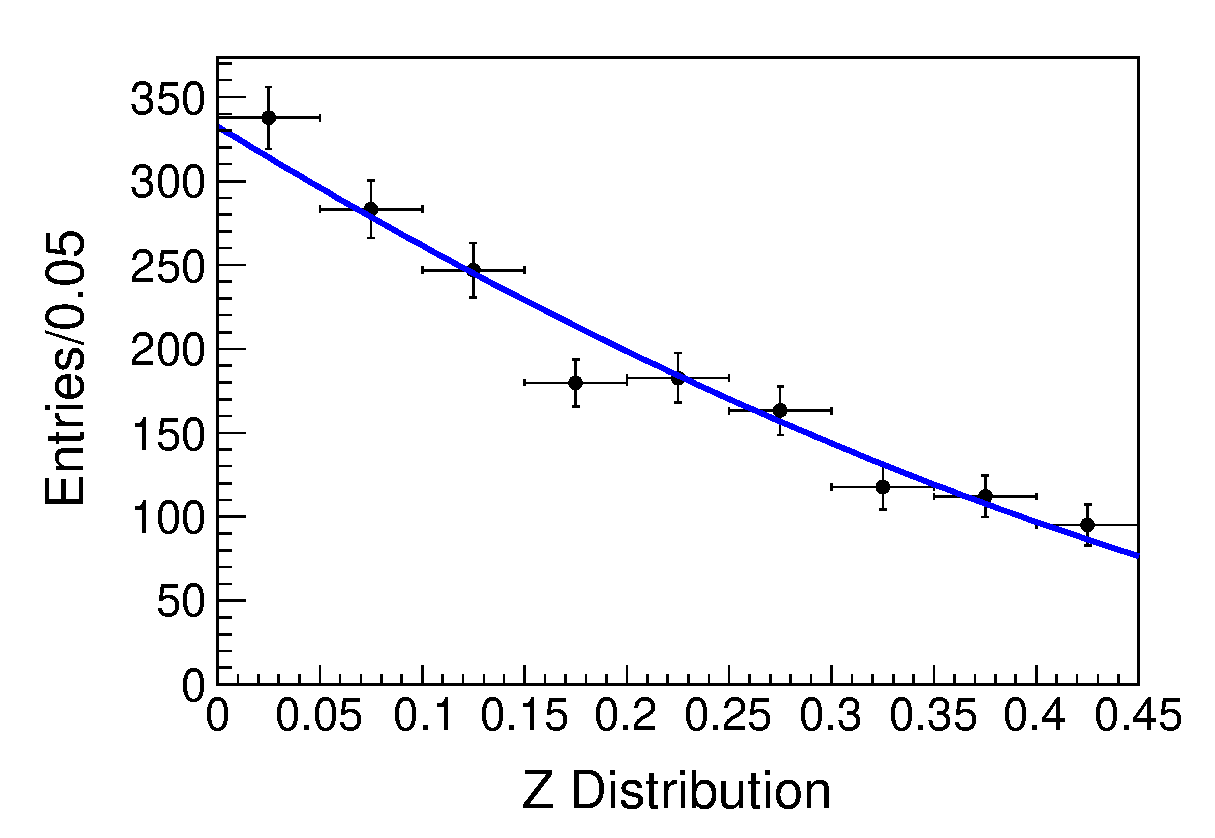
\includegraphics[width=0.5\textwidth]{figures/etapneu/etapneu_dalfit.eps}
    \caption{\label{fig:fitalpha_data_etapneu}Fitting Results of Data}
\end{figure}

\section{SYSTEMATIC ERROR}
Systematic errors for $\eta\ra\pip\pim\pio$ is mainly from resources listed below:
\begin{itemize}
        \item Fitting bias:We can get such source contribution via pull distribution.
        \item Resolution: To estimate the experimental systematic error due to the resolution of X and Y, the resolution functions are numerically convoluted with the p.d.f. while fitting to the data without considering the correlation between X and Y variables. The variations from the nominal values are taken as the systematic uncertainty.
        \item Efficiency: The systematic uncertainty from efficiency includes two terms: the parametrization of efficiency and the difference between data and MC (tracking efficiency, $\pio$ efficiency and $\eta$ constraint).
\end{itemize}
All the errors are summarized in Tab.~\ref{tab:etacha_syserr}. Assuming all the sources are independent and adding them in quadrature, we can get the total systematic errors for the matrix elements shown in the last row in Tab.~\ref{tab:etacha_syserr}.

\begin{table}[!htbp]
 \begin{center}
 \begin{small}
 \caption{\label{tab:etacha_syserr} The systematic errors of the matrix elements.}
 \begin{tabular}{ccccccc}\hline\hline
  	Source 		        &    a(\%)  & b(\%)      & c(\%)     & d(\%)     & e(\%)       & f(\%) \\ \hline
   	Fitting bias        &   0.63    &2.08        & 44.93     & 1.60      & 24.01       & 7.69  \\
   	Resolution          &  0.01     & 0.22       & 3.42      & 0.04      & 0.05        & 0.05 \\
   	$\eta$ constraint   &  0.38     & 1.60       & 794.19    & 2.07      & 12.26       & 12.93 \\
   	Efficiency Para.    &  1.30     & 2.87       & 485.85    & 7.91      & 13.07       & 14.65 \\
   	Tracking efficiency &  0.08    & 0.61       & 101.01    & 0.16      & 2.91        & 0.10 \\
    $\pio$ efficiency 	&  0.05     & 2.01       & 11.85     & 1.66      & 2.99        & 1.3 \\
   	Background shape    &  -        &  -         & -         & -         & -           & - \\
	\hline
    Sum in quadrature   &  1.49     & 4.43       & 937.64    & 8.49      & 30.25       & 21.04  \\
\hline\hline
\end{tabular}
\end{small}
\end{center}
\end{table}

Systematic errors for decay $\eta\ra\pio\pio\pio$ mainly from sources list below:
\begin{itemize}
    \item Efficiency: As those for decay $\eta\ra\pip\pim\pio$, such contributions also includes two terms, one
    is from efficiency parametrization and one is from $\pio$ detection efficiency.
    \item $\eta$ constraint: We use 7C kinematic fit information to calculate the Dalitz
    plot variable $\alpha$ and corresponding fit is performed. The difference on the
    fitted parameter are taken as the systematic error. Such contribution is 3.84\%.
    \item All sources of systematic uncertainties are listed in Table~\ref{tab:etaneu_syserr}.
\end{itemize}

\begin{table}
  \centering
  \caption{\label{tab:etaneu_syserr}Systematic Uncertainties of the slope parameter}
\scriptsize
\begin{center}
\begin{small}
 \begin{tabular}{lrrr}\hline\hline
 	Source & Systematic Uncertainty(\%)\\\hline
	Efficiency Parametrization & 0.41\\
	$\pio$ Efficiency & 3.67\\
	Fit Range & 3.74\\
	$\eta$ constraint & 3.84\\
	Fitting Bias & 6.00\\\hline
	Total & 8.86\\\hline
\hline\hline
\end{tabular}
\end{small}
\end{center}
\end{table}

Sources contributes to decay $\etap\ra\pio\pio\pio$ are like those for decay $\eta\ra\pio\pio\pio$
and some more sources should be considered:
\begin{itemize}
    \item Non-peaking Background: Alter side band ranges, such contribution is 1.45\%.
	\item Peaking Background Branching Fraction:\\
	Since our peaking background events number is normalized to its branching ratio, change
	the input branching ratio value of decay $\etap\ra\eta\pio\pio$ one sigma and we can
	obtain such systematic error contribution as 0.52\%.
	\item Peaking Background Shape:\\
	Using another set of parameters mentioned in Ref.~\cite{PeakDal},
	take the difference as our systematic uncertainty(0.35\%).
	\item All sources of systematic contributions are listed in Table~\ref{tab:etapneu_syserr}.
\end{itemize}

\begin{table}
  \centering
  \caption{\label{tab:etapneu_syserr}Systematic uncertainties of $\eta'\to\pio\pio\pio$}
\scriptsize
%\large
\begin{center}
\begin{small}
 \begin{tabular}{lrrr}\hline\hline
 	Sources & Systematic Uncertainty(\%)\\\hline
	Efficiency Parametrization & 0.90\\
	$\pio$ Efficiency & 1.31\\
	Fit Range & 3.64\\
	Fitting Bias & 2.88\\
	Non-peaking Bg. & 1.45\\
	Peaking Bg. Br. & 0.52\\
	Peaking Bg. Shape & 0.35\\\hline
	Total & 5.16\\\hline
\hline\hline
\end{tabular}
\end{small}
\end{center}
\end{table}

\end{document}
